\section{Simulink Grafiken}

\subsection{Export Funktion}
�ber \mcode{print_mdl('system','testbench_v01','format','pdf');} k�nnen Simulink Modelle direkt in PDFs gewandelt werden.

\subsection{Beispiel}
Guggst du Grafik (Abbildung \ref{img:simulink_waag}) auf Seite \pageref{img:simulink_waag}.

\begin{figure}
	\centering
	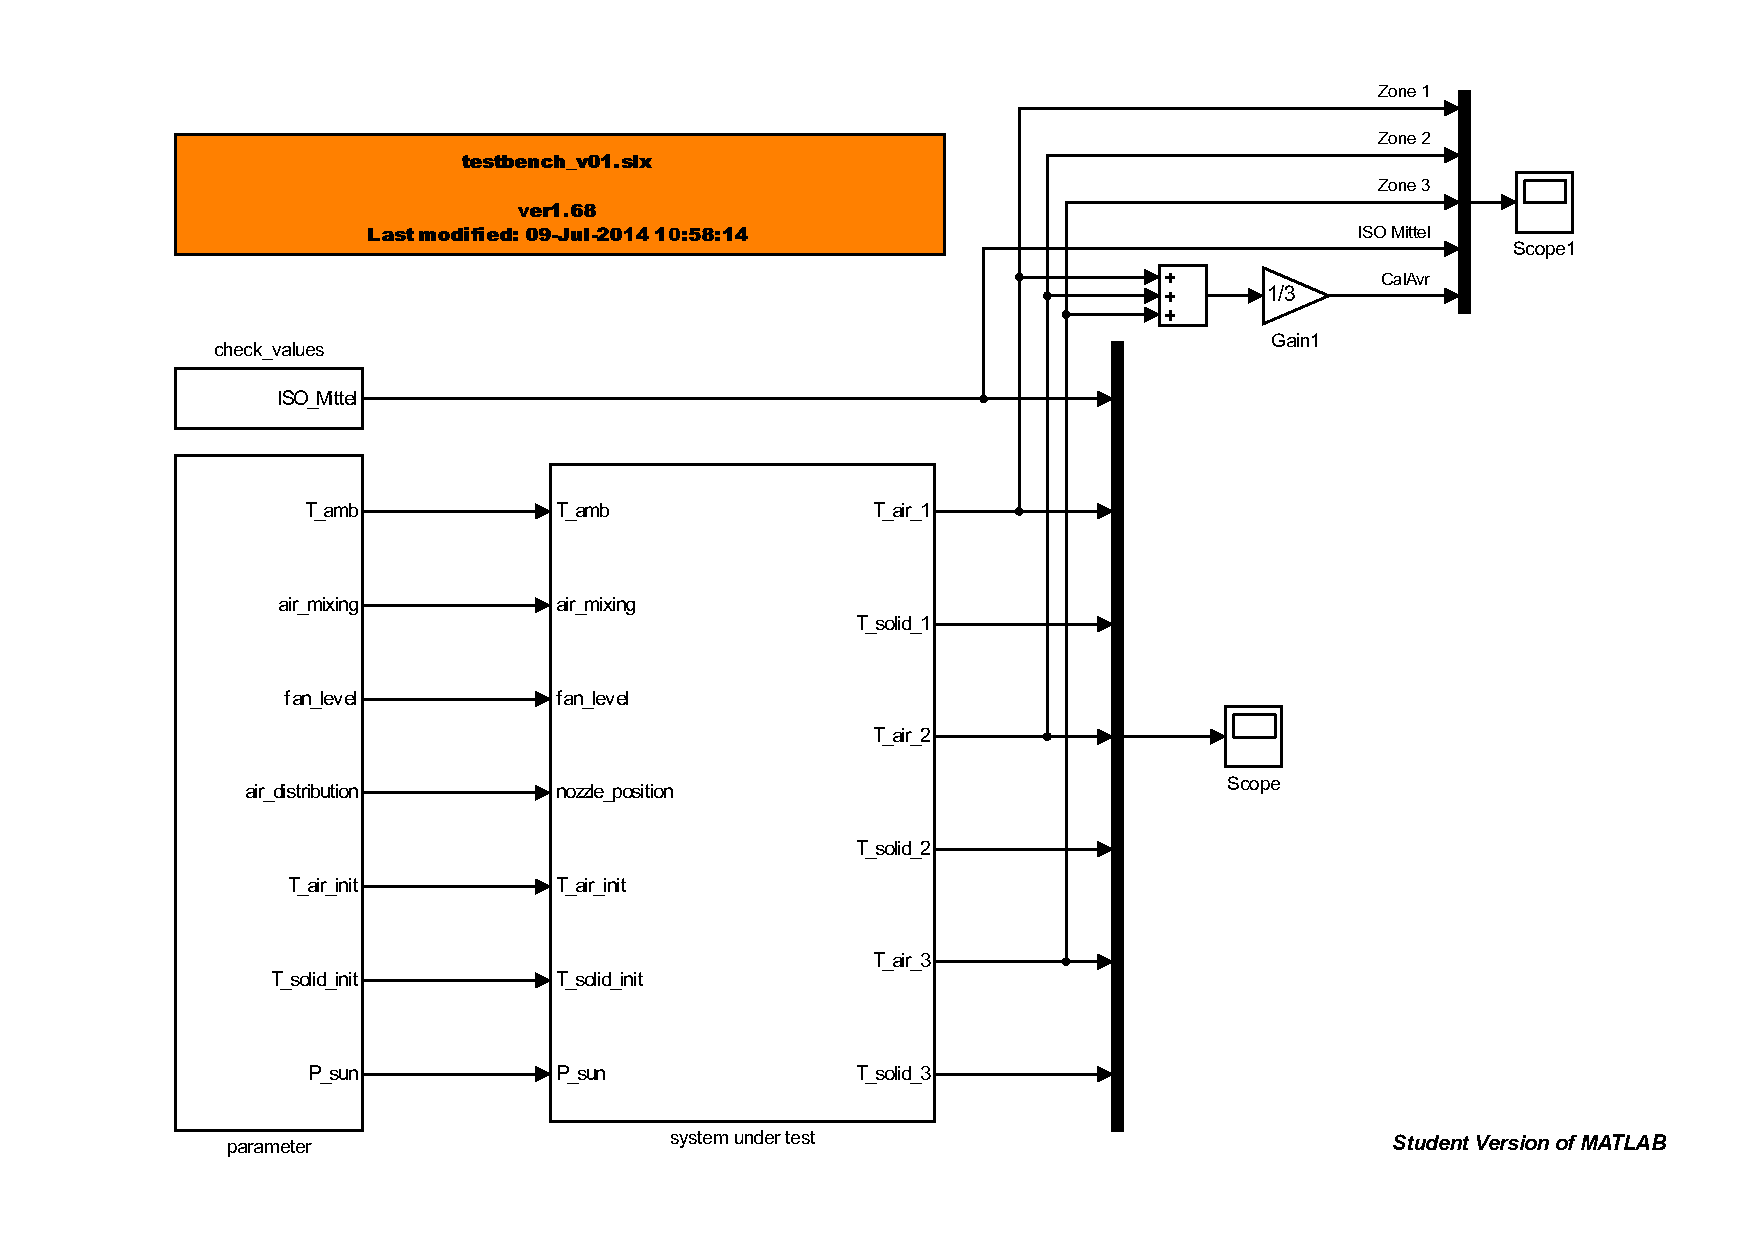
\includegraphics[width=\textwidth]{chapter3/1_gesamt/testbench_v01.pdf}
	\caption{Simulink Modell waagrecht}
	\label{img:simulink_waag}
\end{figure}

\subsection{Gedreht}
Dieselbe Grafik (Abbildung \ref{img:simulink_senk}) gibt es auf Seite \pageref{img:simulink_senk}.
\begin{figure}
	\centering
	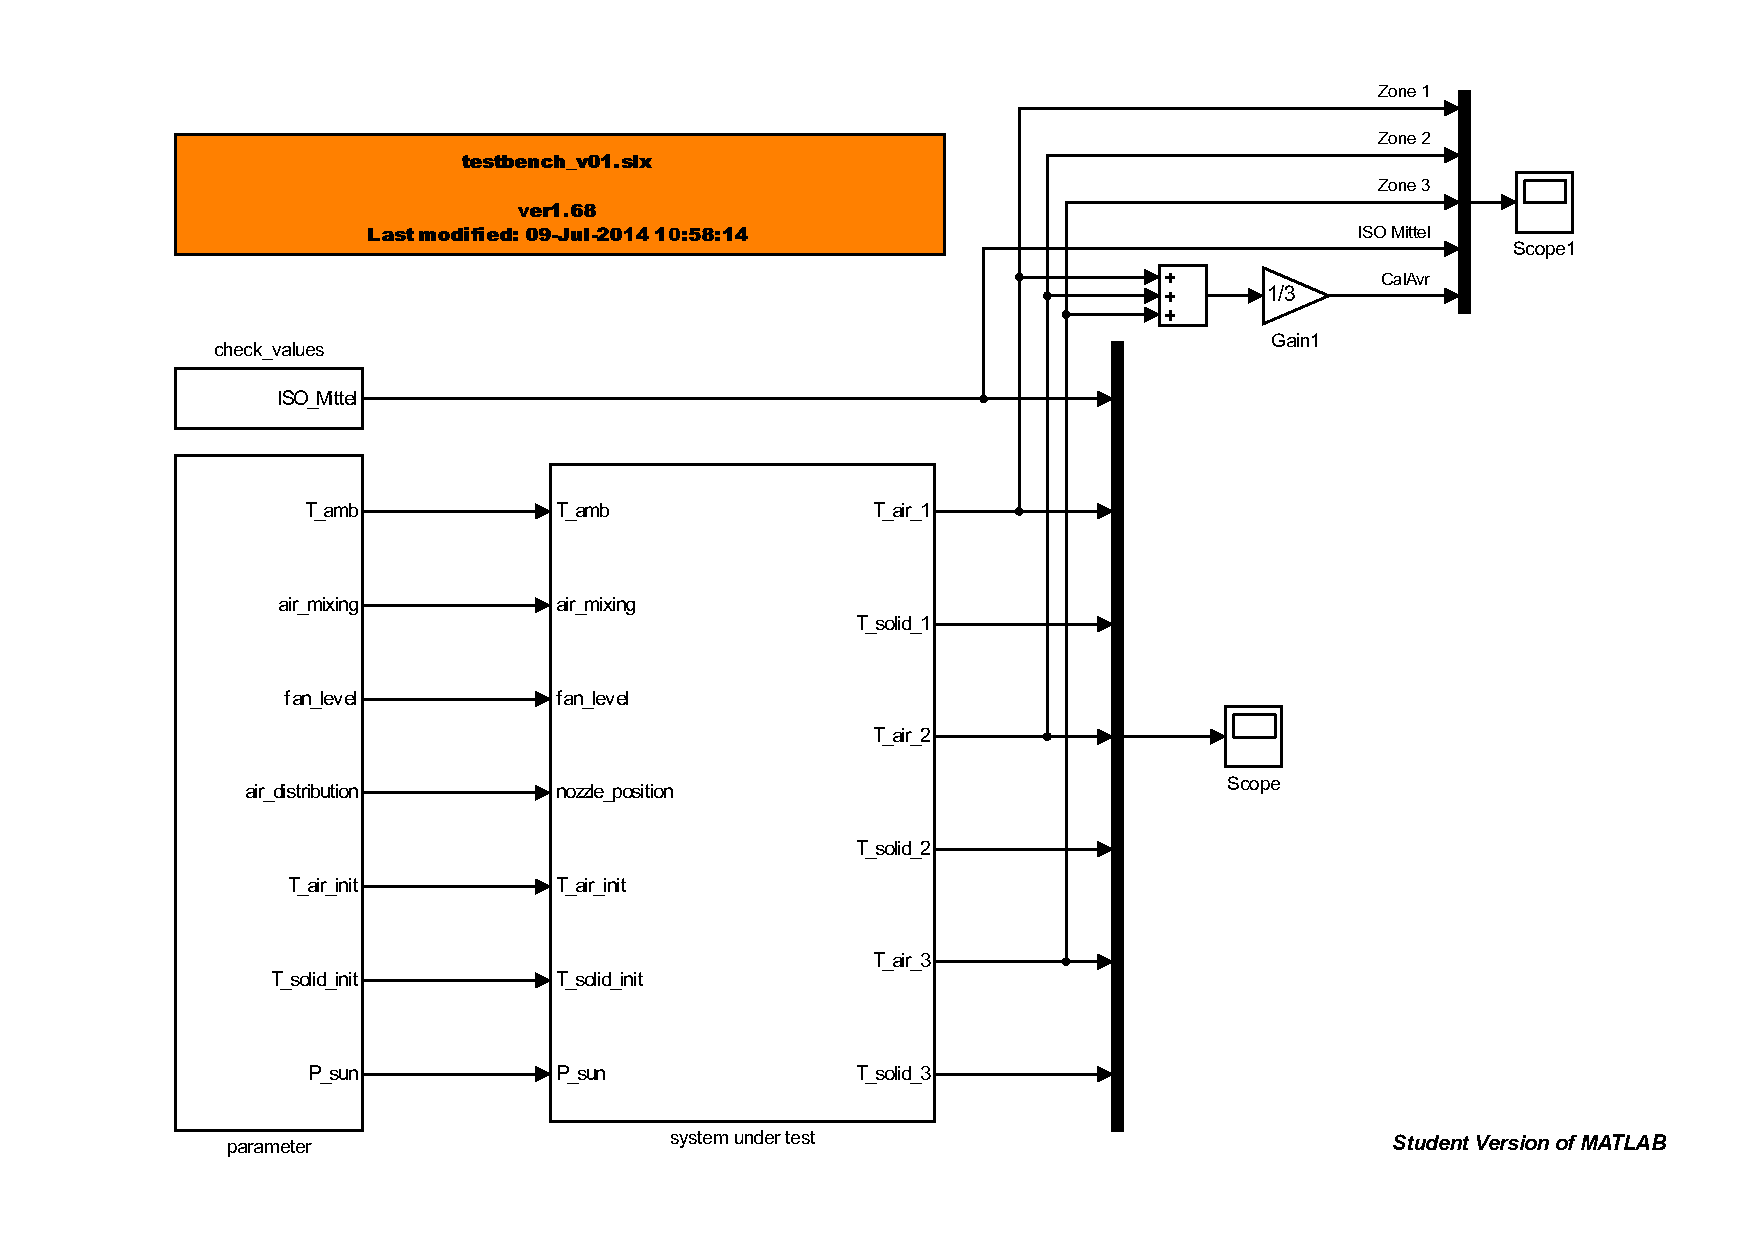
\includegraphics[height=\textwidth,angle=90]{chapter3/1_gesamt/testbench_v01.pdf}
	\caption{Simulink Modell senkrecht}
	\label{img:simulink_senk}
\end{figure}
